\documentclass[10pt]{beamer}

\usetheme{Warsaw}

\usepackage[T1]{fontenc}
\usepackage[utf8]{inputenc}
\usepackage[frenchb]{babel}
\usepackage{graphicx}

\title[Qualité Logicielle]{\bf{Qualité Logicielle}}
\author[CARBONNEL Jessie - LY Julie]{CARBONNEL Jessie - LY Julie}
\institute{Université de Montpellier II}
\date{15 novembre 2012}





\AtBeginSection[]
{
\begin{frame}{Sommaire}
\tableofcontents[currentsection,currentsubsection]
\end{frame}
}


\begin{document}

\begin{frame}
    \titlepage
\end{frame}


\begin{frame}
    \frametitle{Sommaire}
    \tableofcontents              
\end{frame}


% -------- INTRODUCTION ----------------------------------------------
\section{Introduction}


% Définition
\small \subsection{Qu'est-ce que la qualité logicielle ?}

% -----
\begin{frame}
\frametitle{Qu'est-ce que la qualité logicielle ?}

\pause[2] \begin{block}{AFNOR : Qualité}
	Aptitude d’un produit ou d’un service à satisfaire les besoins des utilisateurs.
\end{block}

\bigskip

\pause[3] Appréciation globale basée sur : 
\begin{itemize}
\item<4->De nombreux indicateurs, 
\item<5->Des facteurs extérieurs (clients), 
\item<6->Des facteurs intérieurs (développeurs). 
\end{itemize}

\bigskip

\pause[7] Une bonne qualité logicielle, mais dans quel but ? 
     \begin{itemize}
     \item<8->Certifier aux utilisateurs que le logiciel est conforme.
     \item<9->\'Eviter aux entreprises (eBay, Facebook, ...) des pertes financières.
     \item<10->Domaines sensibles (militaire, médical, ...) : \'Eviter les pertes humaines. 
\end{itemize}

\end{frame}

% -----
\begin{frame}
\frametitle{Exemples de négligence de la qualité...}

\pause[2] \begin{exampleblock}{ Indisponibilité des serveurs d'Ebay }
     \begin{itemize}
     \item<3->Le 10 juin 1999, indisponibilité des serveurs durant 22h.
     \item<4->\'Echec de plus de 2,3 millions d'enchères.
     \item<5->Ebay doit rembourser pour plus de 3M de dollars...
     \end{itemize}
\end{exampleblock}

\pause[6] \begin{exampleblock}{ Grave incident de radiothérapie à l'hôpital d'\'Epinal (France) }
     \begin{itemize}
     \item<7->Erreur de programmation d'un système de paramétrage.
     \item<8->24 patients atteints d'un cancer surirradiés à plus de 20\%
     \item<9->5 patients morts...
     \end{itemize}
\end{exampleblock}

\pause[10] \begin{alertblock}{}
 \alert{La qualité logicielle n'est donc certainement pas à négliger !}
\end{alertblock}

\end{frame}


% Première apparition
\subsection{Première apparition}

\begin{frame}
\frametitle{Première apparition}

\begin{enumerate}
\pause[2] \item Apparition de la "Crise Logicielle" vers 1960.
	\begin{itemize}
	\item<3->\smallskip Une réponse à cette crise ?
	\end{itemize}
\item<4-> \bigskip Création du Génie Logicielle en 1968.
	\begin{itemize}
	\item<5->\smallskip Peut-on faire encore mieux ?
	\end{itemize}
\item<6->\bigskip Pourquoi ne pas normaliser tous les logiciels ?
\end{enumerate}

\end{frame}


% Organisation de normalisation
\subsection{Organisation de normalisation}
\begin{frame}
\frametitle{Définitions}
\pause[2] \begin{block}{Norme}
	Une norme est un ensemble de caractéristiques décrivant et régissant un domaine particulier un objet, un produit, un être.
\end{block}

\bigskip

\pause[3] \begin{block}{Organisme de normalisation}
	Organisme dont les activités premières sont l'établissement puis le maintien de normes.
\end{block}

\end{frame}

\begin{frame}
\frametitle{Organisation de normalisation}
\pause[2] En 1947, création de l'ISO (International Organization for Standardization) :
   \begin{itemize}
	\item<3-> Composée de 164 organisations nationales de normalisation.
	\item<4-> Producteur de normes internationales (normes ISO).
    \end{itemize}

\bigskip

\pause[5] Plus de 19000 normes actives, dont :
   \begin{itemize}
	\item<6-> La norme ISO9126
	\item<7-> La norme ISO14598
    \end{itemize}
\end{frame}



% -------- Les normes ----------------------------------------------
\section{Les normes}

% ISO9126
\subsection{La norme ISO9126}
\begin{frame}
\frametitle{Qu'est-ce que la norme ISO9126 ?}

\pause[2] \textbf{La norme ISO9126 :}
\medskip
   \begin{itemize}
	\item<3-> Une norme parmi l'ensemble des ISO9000.
\medskip
		   \begin{itemize}
			\item<4-> Gestion de la qualité.
    		   \end{itemize}
\medskip
	\item<5-> Propose un modèle de qualité logicielle.
\medskip
	\item<6-> Pose les caractéristiques principales d'un logiciel.
    \end{itemize}

\end{frame}

%
\begin{frame}
\frametitle{Les principales caractéristiques}
\pause[2]Les 6 caractéristiques principales de la norme ISO9126 :
	\begin{itemize}
	\item<3->Capacité fonctionnelle,
	\item<4->Fiabilité,
	\item<5->Facilité d'utilisation,
	\item<6->Rendement,
	\item<7->Maintenabilité,
	\item<8->Portabilité.
	\end{itemize}
\end{frame}

%
\begin{frame}
\frametitle{Les dérives}
\pause[2] \textbf{Capacité fonctionnelle :}
	\begin{itemize}
	\item<3->Aptitude,
	\item<4->Exactitude,
	\item<5->Interopérabilité,
	\item<6->Sécurité.
	\end{itemize}

\medskip

\pause[7] \textbf{Fiabilité :}
	\begin{itemize}
	\item<8->Maturité,
	\item<9->Tolérance aux fautes,
	\item<10->Possibilité de récupération.
	\end{itemize}

\medskip

\pause[11] \textbf{Facilité d'utilisation :}
	\begin{itemize}
	\item<12->Facilité de compréhension,
	\item<13->Facilité d'apprentissage,
	\item<14->Facilité d'exploitation.
	\end{itemize}
\end{frame}

\begin{frame}
\frametitle{Les dérives [suite]}
\pause[2] \textbf{Rendement :}
	\begin{itemize}
	\item<3->Comportement face au temps,
	\item<4->Comportement face aux ressources.
	\end{itemize}

\medskip

\pause[5] \textbf{Maintenabilité :}
	\begin{itemize}
	\item<6->Facilité d'analyse,
	\item<7->Facilité de modification,
	\item<8->Stabilité,
	\item<9->Facilité de test.
	\end{itemize}

\medskip

\pause[10] \textbf{Portabilité :}
	\begin{itemize}
	\item<11->Facilité d'adaptation,
	\item<12->Facilité d'installation,
	\item<13->Conforme aux règles de portabilité,
	\item<14->Interchangeabilité.
	\end{itemize}
\end{frame}

%
\begin{frame}
\frametitle{A savoir !}

   \pause[2] \begin{center}
	\alert{Certaines de ces caractéristiques sont conflictuelles entre elles !}
   \end{center}

\medskip

   \pause[3] \begin{center}
	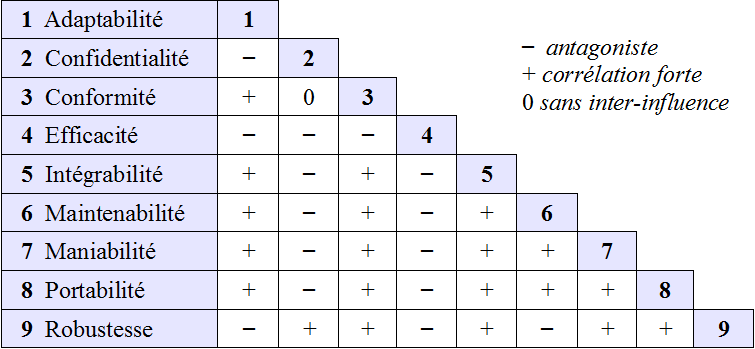
\includegraphics[scale=0.4]{tableau.png} \\
	\textit{"Tableau des intéractions entre les aptitudes d'un logiciel"} \\
		\smallskip
	\tiny{\textbf{Source :} "La démarche objet : concept et outils" (Max Bouché, Ed. Afnor) }
   \end{center}

\end{frame}



% ISO14598 -----
\subsection{La norme ISO14598}
\begin{frame}
\frametitle{Qu'est-ce que la norme ISO14598 ?}
\pause[2] \textbf{La norme ISO14598 :}
\medskip
   \begin{itemize}
	\item<3-> \'Evalue les caractéristiques de la qualité.
\smallskip
		   \begin{itemize}
			\item<4->Comment ?
    		   \end{itemize}
    \end{itemize}

\bigskip

\pause[5] \textbf{Mise en place d'un processus d'évaluation :}
\smallskip
   \begin{itemize}
	\item<6-> Définition des exigences de qualité,
\smallskip
	\item<7-> Préparation de l'évaluation,
\smallskip
	\item<8-> Procédure d'évaluation.
    \end{itemize}
\end{frame}

\begin{frame}
\frametitle{Description des différentes étapes}
   \begin{itemize}
	\item<2-> Définition des exigences de qualité :
		   \begin{itemize}
			\item<3->Déterminer les caractéristiques à mettre en avant. \\
			\pause[4]\textit{Exemple : Traiter beaucoup de données rapidement : Efficacité.}
    		   \end{itemize}
\medskip
	\item<5-> Préparation de l'évaluation :
		   \begin{itemize}
			\item<6->Sélectionner les indicateurs de qualité. \\
			\pause[7]\textit{Exemple (suite) : Efficacité -> mesure de la complexité.}
\smallskip
			\item<8->Définir un taux de satisfaction à chaque exigence.
\smallskip
			\item<9->Définir des critères d'appréciation.
    		   \end{itemize}
\medskip
	\item<10-> Procédure d'évaluation :
		   \begin{itemize}
			\item<11->Mesure des indicateurs.
\smallskip
			\item<12->Note de satisfaction pour chaque mesure.
\smallskip
			\item<13->\'Evaluer le produit final.
    		   \end{itemize}
    \end{itemize}
\end{frame}



% -------- Conclusion ----------------------------------------------
\section{Un peu plus loin}

%
\subsection{Vers une nouvelle norme ISO ?}
\begin{frame}
\frametitle{Vers une nouvelle norme ISO ?}
\pause[2] La norme ISO25000 :
\medskip
   \begin{itemize}
	\item<3-> Appelée SQuaRE (Software Quality Requirements and Evaluation).
\medskip
	\item<4-> Concerne l'exigence qualité/évaluation d'un produit logiciel.
\medskip
	\item<5-> Plus précis que l'ISO9126.
\medskip
	\item<6-> Accompagnée de guides détaillés.
\medskip
	\item<7-> Devrait remplacer les normes ISO9126 et ISO14598.
    \end{itemize}
\end{frame}




% -------- Sources ----------------------------------------------
\section{Sources}

\begin{frame}
\frametitle{Sources}
{\large \textbf{Livres :} }
     \begin{itemize}
     \item "La démarche objet : Concept et outils" (Max Bouché, Ed. Afnor)
     \item "L'ingénierie des systèmes d'information évolutifs" (Serge Bouchy, Ed. Eyrolles)
     \end{itemize}

\bigskip

{\large \textbf{Sites :} }
     \begin{itemize}
     \item www.wikipedia.fr
     \item www.lefigaro.fr
     \item www.techniques-ingenieur.fr
     \item www.numeraladvance.com
     \item www.sikora.fr
     \end{itemize}
     
\end{frame}




\end{document}
